\documentclass{article}
\usepackage[paper=letterpaper,margin=2cm]{geometry}
\usepackage[russian]{babel}
\usepackage[utf8]{inputenc}
\usepackage[]{graphicx}
\usepackage[usenames]{color}
\usepackage{colortbl}
\usepackage{geometry}
\usepackage{xcolor}
\usepackage{listings}

\geometry{
  a4paper,
  top=25mm, 
  right=30mm, 
  bottom=25mm, 
  left=30mm
}

\begin{document}

\begin{center}
  \section*{
    Федеральное государственное автономное образовательное учреждение\\ высшего образования\\
    «Национальный исследовательский университет ИТМО»\\
    Факультет Программной Инженерии и Компьютерной Техники \\
   }
  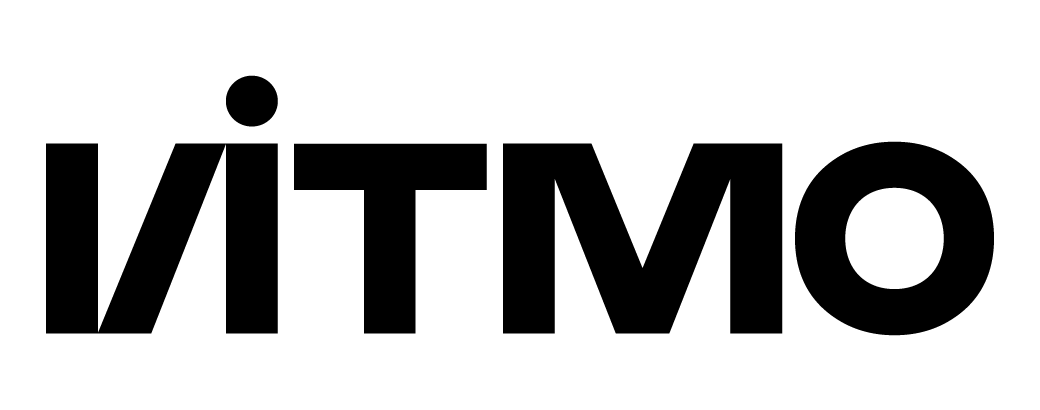
\includegraphics[scale=0.2]{../../img/itmo.png}
\end{center}
\vspace{4cm}


\begin{center}
  \large \textbf{Вариант \textnumero 666}\\
  \textbf{Лабораторная работа \textnumero 1}\\
  по дисциплине\\
  \textbf{Программирование}
\end{center}

\vspace*{\fill}

\begin{flushright}
  Выполнил Студент группы P3115\\
  \textbf{Владимир Мацюк}\\
  Преподаватель: \\
  \textbf{ФИО препода}\\
\end{flushright}

\vspace{1cm}

\begin{center}
  г. Санкт-Петербург\\
  2022г.
\end{center}

\newpage

\lstset{
  inputencoding=utf8,
  frame=single,
  language=Java,
  breaklines=true,
  extendedchars=false,
  showspaces=false,
  showstringspaces=false,
  basicstyle=\footnotesize\ttfamily,
  keywordstyle=\bfseries\color{green!40!black},
  commentstyle=\itshape\color{purple!40!black},
  identifierstyle=\color{blue},
  stringstyle=\color{orange},
}

\section*{Цель работы}

\section*{Ход работы}

\lstinputlisting{Lab1.java}

\section*{Вывод}

\end{document}
